\section{Prüfung 28.05.2021}
\subsection{Profit / Penalty}
\subsubsection{a)}
Wir betrachten die Servolenkung eines PKW. Ab dem Zeitpunkt wo der Fahrer das Lenkrad bewegt
sollen höchstens 50ms vergehen bis der Stellmotor der Servolenkung die Räder in den gewünschten
Stellwinkel gebracht hat.
Zeichnen Sie in das folgende Diagramm den Profit/Penalty-Verlauf für die Servolenkung ein, d.h. zum
Zeitpunkt t soll der Profit bzw. Penalty-Wert für den Fall eingetragen werden, dass der Stellmotor zum
Zeitpunkt t den Stellvorgang der Räder beendet. Gehen Sie dabei davon aus, dass der Fahrer das
Lenkrad zum Zeitpunkt 0ms bewegt hat.
\begin{figure}[H]
  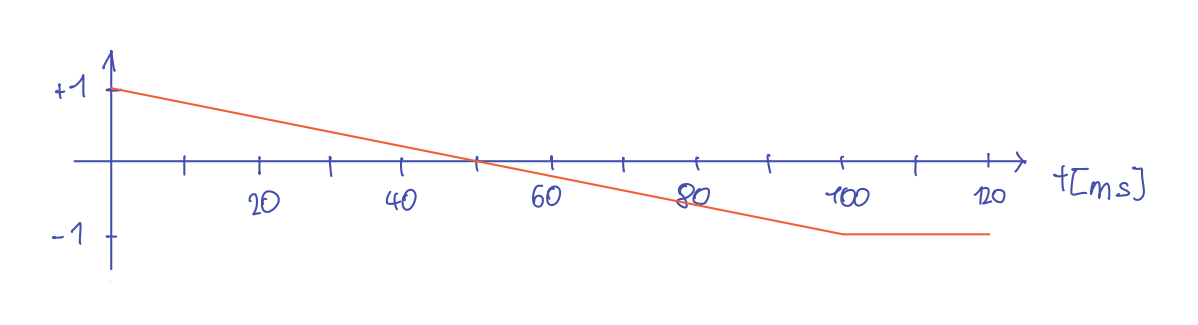
\includegraphics[width=10cm]{images/KA280521/1a.PNG}
  \centering
\end{figure}

\subsubsection{b)}
Handelt es sich hier um weiche, feste oder harte Echtzeit? Begründen Sie!

Es handelt sich hier um harte Festzeit. Werden die Räder nicht bis zu der Deadline in die richtige Stellung gebracht 
kann es durch einen Unfall zu Schäden kommen.

\subsection{Echtzeitbusse}
\subsubsection{a)}
Im Gegensatz zum I2C-Bus verfügt der CAN-Bus über keine Taktleitung. Welches Problem entsteht
dadurch und wie wird es beim CAN-Bus gelöst?

Die Geräte kennen den Takt der anderen Geräte nicht und somit kommt es zu einem Synchronisationsproblem. Dieses wird durch 
Stuff Bits gelöst. Werden fünf gleich wertige bits gesendet wird ein stuff bit mit gegenwertiger Wertigkeit gesendet um den Takt 
zu synchronisieren.

\subsubsection{b)}
Worin liegt der Unterschied zwischen dem Adressfeld in I2C Nachrichten und dem „Identifier“ in
CAN Nachrichten?

In einem Adressfeld steht immer nur eine Adresse eines Gerätes welches eine Nachricht senden oder empfangen soll.
Bei CAN kann jeder der sich als derjenige „Identifier“ identifiziert von der Nachricht lesen.

\subsubsection{c)}
Ist der I2C-Bus bei Vorhandensein von einem Master und mehreren Slaves hart echtzeitfähig? Begründen Sie Ihre Antwort!

Nein. Aufgrund der Prioritätsaufteilung ist I2C nicht hart echzeitfähig. Niedrigere Adressen haben höhere Priorität und 
Adressen können oft nicht willkürlich gewählt werden.

\subsubsection{d)}
Welche technischen Eigenschaften von Ethernet führen dazu, dass es nicht echtzeitfähig ist?

Aufgrund von der CSMA/CD Methode und TCP/IP Protokoll hat Ethernet keine Echtzeitfähigkeit.
Verzögerungen durch Collision Detection. Konflikte und Überlastungen am Übertragungskanal. 

CSMA/CD (\textbf{C}arrier \textbf{S}ense \textbf{M}ultiple \textbf{A}ccess / \textbf{C}ollision \textbf{D}etection).

Real-Time Ethernet (RTE) wäre ein alternative.

\subsection{Task-Synchronisation}
Gegeben seien zwei Tasks T1 und T2. Zuerst soll T1 Calc1() ausführen, nachdem diese Funktion beendet ist
sollen T1 und T2 die Funktionen Calc2() und Calc3() (quasi) gleichzeitig ausführen.

\subsubsection{a)}
\begin{figure}[H]
  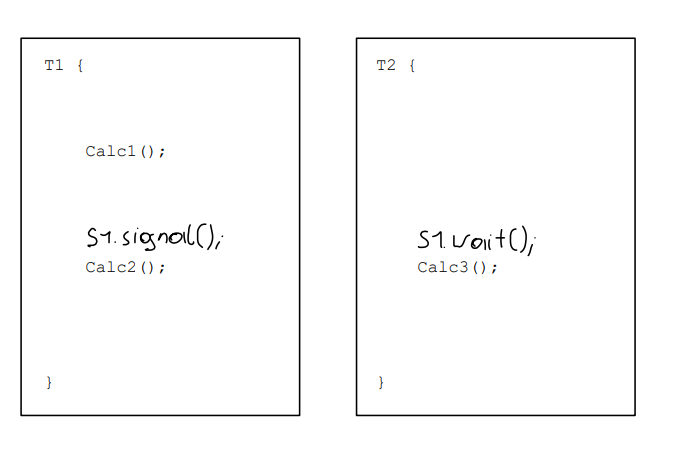
\includegraphics[width=10cm]{images/KA280521/3a.PNG}
  \centering
\end{figure}

\subsubsection{b)}
S1 muss mit 0 intialisiert werden!

\subsection{Echtzeitscheduling}
Die Abbildung zeigt das Schedule für die Ausführung der folgenden Tasks T1, T2, T3 auf einem Prozessor.
T1 = (X; 4), T2 = (1; 5), T3 = (3; 10)
wobei ein Task als Tn = (Ausführungszeit; Periode) definiert ist. Für jeden Task ist die Periode identisch mit
der Deadline. Die Ausführung aller Tasks beginnt gleichzeitig zum Zeitpunkt 0.
\begin{figure}[H]
  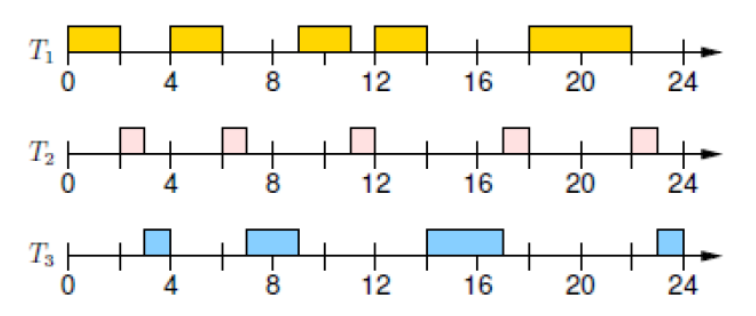
\includegraphics[width=10cm]{images/KA280521/4a.PNG}
  \centering
\end{figure}

\subsubsection{a)}
Wie groß ist die Worst-Case Execution Time X von Task T1? Begründen Sie!

$X=2$, da bei T1 innerhalb von einer Periode (=4 Zeitschritten) die Ausführungszeit immer 2 ist.

\subsubsection{b)}
keine Ahnung.

\subsection{Statecharts}
Der folgende Programmcode wurde aus einem Statechart generiert. Zeichnen Sie den ursprünglichen
Statechart, tragen Sie auch die Namen aller Zustände sowie aller Ereignisse ein und markieren Sie alle
initialen Zustände so wie in Statecharts üblich!

\begin{lstlisting}
#define Q 1
#define R 2
#define S 3
#define T 4
void main () {
  int state = Q;
  while (1) {
    int a = update_a();
    int b = update_b();
    int c = update_c();
    switch (state) {
      case Q: if (b) { state = R; }
                else if (c) { state = T; } break;
      case R: if (a) { state = S; } break;
      case S: if (b) { state = R; } break;
      case T: if (a) { state = Q; } break;
    }
  }
}
\end{lstlisting}

\begin{figure}[H]
  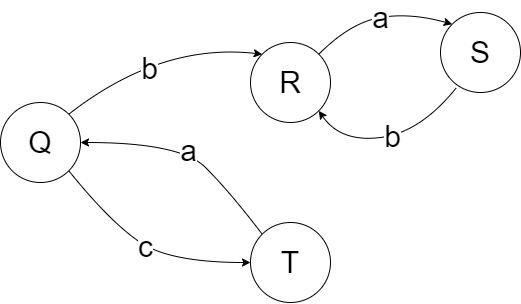
\includegraphics[width=10cm]{images/KA280521/5a.PNG}
  \centering
\end{figure}

\subsection{Speicherprogrammierbare Steuerungen}

\subsubsection{a)}
Definieren Sie die Begriffe Eingabezeit, Zykluszeit und Reaktionszeit bei einer SPS!

\begin{itemize}
  \item Eingabezeit: Eingänge werden gelesen und in das Prozessabbild geschrieben.
  \item Zykluszeit: Zykluszeit = Eingabezeit + Verarbeitungszeit + Ausgabezeit. 
  \item Reaktionszeit: bezieht sich auf die Zeit, die ein System benötigt, um auf eine Änderung im Eingangssignal zu reagieren.
\end{itemize}

\subsubsection{b)}
Wie groß ist die minimale Reaktionszeit einer SPS? Begründen Sie!

\begin{equation}
  t_{rmin} = t_i + t_c + t_o
\end{equation}

\begin{equation}
  t_{rmax} = t_i + 2\cdot t_c + t_o
\end{equation}


\subsubsection{c)}
Geben Sie für folgenden strukturierten Text einen äquivalenten Kontaktplan (KOP) an: B = ((NOT A)
AND C) OR D

\begin{figure}[H]
  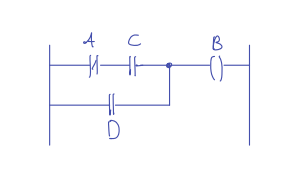
\includegraphics[width=10cm]{images/KA280521/6c.PNG}
  \centering
\end{figure}